\documentclass[letterpaper,12pt]{article}
\usepackage[margin=64pt]{geometry}
\usepackage{amsthm}
\usepackage{amsmath}
\usepackage{amssymb}
\usepackage{parskip}
\usepackage{graphicx}
\usepackage{enumerate}
\usepackage{hyperref}
\usepackage{listings}
\newcommand{\transpose}{^{\mbox{\tiny T}}}


\begin{document}
\thispagestyle{empty}

\hrule \vspace{0.5em}
\noindent {\bf CFRM 461: Probability and Statistics for Computational Finance} \hfill Homework 1 \newline \hrule

\vspace{1em}
\textbf{Instructions:} Please round your answers to 2 decimal places unless stated otherwise. Since R codes in this homework are simple, please paste them directly in your write-up. There is NO need to upload separate R files for this homework.

\begin{enumerate}

%Q1
\item A Seattle hospital is concerned about the rising number of low birth weight of babies. They then collected data on the mother's age, the mother's pre-pregnancy weight, the level of pre-natal care (none, minimal, adequate), and whether the mother used drugs during pregnancy (cigarettes, alcohol, etc).
\\\\Note: Please identify the type (categorical or quantitative) for the four variables in the study: "age", "pre-pregnancy weight", "level of prenatal care", and "drug use".

Mothers Age: Quantitative
\\
Pre-pregnancy weight: Quantitative
\\
Pre-natal care: Categorical
\\
Drugs: Categorical

%Q2
\item The results of a survey of automobiles parked in student and staff lots at a large university are listed in the table below.
\begin{table}[h]
\centering
\renewcommand{\arraystretch}{1.2}
\begin{tabular}{|l|cc|} \hline
  & Student & Staff \\ \hline
North American & 91 & 90 \\
European & 31 & 16 \\
Asian & 68 & 54 \\ \hline  
\end{tabular}
\caption{Two-Way Table}
\label{tab1}
\end{table}

\vspace{-1em}
We name the two variables in Table \ref{tab1} by ``Driver" and ``Origin" (both are categorical variables). The ``Driver" variable has two categories: ``Student" and ``Staff", while the ``Origin" variable has three categories: ``North American", ``European", and ``Asian".

\textbf{Hints}: A distribution gives the probabilities (relative frequency) for all possible outcomes. Please report the probabilities in percentage with two decimal places accuracy (e.g., 12.34\%).

\begin{table}[h]
\centering
\renewcommand{\arraystretch}{1.2}
\begin{tabular}{|l|ccc|} \hline
  & Student & Staff & Total\\ \hline
North American & 91 & 90 & 181\\
European & 31 & 16 & 47 \\
Asian & 68 & 54 & 122\\ \hline
Total & 190 & 160 & 350\\ \hline
\end{tabular}
\caption{Contingency Table}
\label{tab1}
\end{table}
\newpage
\subitem(a) What is the marginal distribution of ``Origin"? 

\begin{table}[h]
\centering
\renewcommand{\arraystretch}{1.2}
\begin{tabular}{|ccc|} \hline
 Origin & Frequency & Relative Frequency (\%)\\ \hline
North American & 181 & 51.72\\
European & 47 & 13.43 \\
Asian & 122 & 34.86 \\\hline
\end{tabular}
\caption{Marginal Distribution}
\label{tab1}
\end{table}

\subitem(b) What is the marginal distribution of ``Driver"?

\begin{table}[h]
\centering
\renewcommand{\arraystretch}{1.2}
\begin{tabular}{|ccc|} \hline
Driver & Student & Staff\\ \hline
Frequency & 190 & 160\\
Relative Frequency (\%) & 54.29 & 45.71\\ \hline
\end{tabular}
\caption{Marginal Distribution}
\label{tab1}
\end{table}

\subitem(c) What is the conditional distribution of ``Origin" for ``Staff"?

\begin{table}[h]
\centering
\renewcommand{\arraystretch}{1.2}
\begin{tabular}{|ccc|} \hline
 Origin & Frequency & Relative Frequency (\%)\\ \hline
North American & 90 & 56.25\\
European & 16 & 10 \\
Asian & 54 & 33.75 \\\hline
\end{tabular}
\caption{Marginal Distribution}
\label{tab1}
\end{table}

\subitem(d) What is the probability (relative frequency) that the driver of a car is a student given that he/she is a North American?

\[\frac{91}{181} \implies 50.27\%\]

%Q3
\item In this \verb=R= programming question, please paste the codes in your write-up, or alternatively, you may use R-markdown to prepare your submission. 

\subitem(a) Create a $3 \times 2$ matrix, named by \verb=M=, to record all the entries in Table 1, i.e., 
\begin{align*}
M = \begin{pmatrix}
91 & 90 \\
31 & 16 \\
68 & 54\\
\end{pmatrix}
\end{align*} 
To receive full credits, you need to provide at least two different methods.

\begin{lstlisting}
	mat <- matrix(c(91,90,31,16,68,54),3,2,TRUE)
\end{lstlisting}
Output :  \begin{align*}
\begin{matrix}
91 & 90 \\
31 & 16 \\
68 & 54\\
\end{matrix}
\end{align*} 
\begin{lstlisting}
	> x <- c(91,31,68)
	> y <- c(90,16,54)
	> cbind(x,y)
\end{lstlisting}
Output :  \begin{align*}
\begin{matrix}
91 & 90 \\
31 & 16 \\
68 & 54\\
\end{matrix}
\end{align*} 

\subitem(b) Find the row sums and the column sums of matrix \verb=M=.

\begin{lstlisting}
	rowSums(mat)
	colSums(mat)
\end{lstlisting}
Output : 181  47 122 \\
Output : 190 160
\subitem(c) Create a bar plot for the variable ``Origin". In the plot, please (1) name the title of the plot as ``Bar Plot of Origin", (2) name all three categories (North American, European, Asian), (3) use frequency (count) as the y-axis and choose [0, 200] as the range of the y-axis. 

In the \verb=barplot()= command, please specify \verb=main=, \verb=names.arg=,  \verb=ylim= as above. Please use \verb+width = 1+ when drawing the barplot.
Please read the help document on \verb=barplot= to understand the meanings of those arguments.

\begin{lstlisting}
origin <- c(181,47,122)
barplot(origin,main = "Bar Plot of Origin", names.arg = 
c("North American","European","Asian"),ylim = c(0,200),ylab = 
"Frequency",xlab = "Origin", width = 1)
\end{lstlisting}
\begin{center}
\includegraphics[scale = 0.5]{barplot}
\end{center}
%Q4
\item The prices of walking shoes in \$ are listed below:
\[ 90, 70, 70, 70, 75, 70, 65, 68, 60, 74, 70, 95, 75, 68, 85, 65 \]

\begin{itemize}
\item[(a)] We use the build-in function \verb=hist()= of \verb=R= to construct a histogram for the given data set through the following steps: 
\begin{enumerate}
\item Create a vector to record all the observations
\item Create a vector for the breakpoints between histogram cells: use 60,  65,  70,  75,  80,  85,  90,  95, 100, i.e., the first bin is [60, 65], the second is (65, 70], etc.
\item Use frequency as the y-axis, and pick the range of [0, 10] for the y-axis
\item Label the x-axis by ``Price", and pick the range of [60, 100] for the x-axis
\item Name the title of the histogram as ``Histogram of Price"
\item Choose \verb=TRUE= for plot option
\end{enumerate}
Please paste the codes and the final histogram in your write-up.

Hints: You need to specify \verb=breaks=, \verb=freq=, \verb=main=, \verb=xlim=, \verb=ylim=, \verb=xlab=, \verb=plot= in the \verb=hist()= command to obtain the desired histogram.

\begin{lstlisting}
	counts <- c(90, 70, 70, 70, 75, 70, 65, 68, 60, 74, 70, 95,
	75,68, 85, 65)
	brk <- c(60,65,70,75,80,85,90,95,100)
\end{lstlisting}
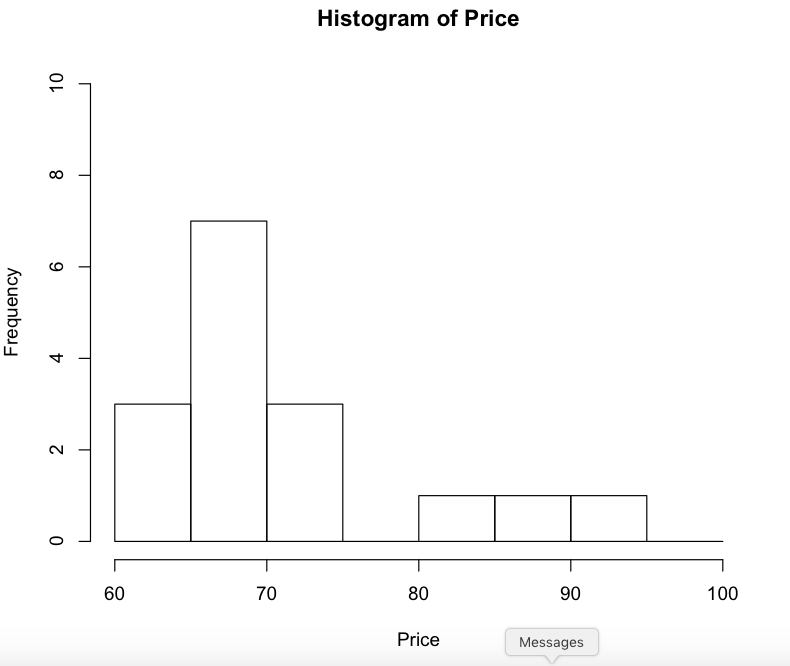
\includegraphics[scale = 0.5]{Hist}

\item[(b)] Identify the shape of the distribution of the shoes price, i.e., identify three features of a distribution: mode (unimodal, bimodal, etc), symmetry (symmetric, skewed to the left/right), and outliers (yes or no).

It is a unimodal distribution that is skewed to the right and contains outliers.

\item[(c)] Compute the mean and the median of the given data set, and compare them to confirm your conclusion on the symmetry feature of the distribution in (b).

\begin{lstlisting}
> mean(counts)
[1] 73.125
> median(counts)
[1] 70
\end{lstlisting}
Clearly the mean > median so the distribution is positively skewed

\item[(d)] Calculate the range, the interquantile range (IQR), and the standard deviation of the given data set.
\end{itemize}

\begin{lstlisting}
> range(counts)
[1] 60 95
counts <- sort(counts)
> IQR <- median(counts[9:16]) - median(counts[1:8])
> IQR
[1] 7
> sd(counts)
[1] 9.372833
\end{lstlisting}

\textbf{Remark}: You may use \verb=R= to calculate Q4 (c) and (d), and if you choose to do so, please paste the codes in your write-up as well.
But please be aware that in the exams you will need to compute those by hands.

%Q5
\item 
\begin{itemize}
\item[(a)] The volumes of soda in 1 litre cola bottle can be described by a Normal model with a mean of 0.95 L and a standard deviation of 0.04 L. What percentage of bottles can we expect to have a volume less than 0.94 L?

\[
	z = \frac{y-\bar{y}}{s} 
\]
\[
	\implies \frac{0.94-0.95}{0.04} = -0.25
\]
\[
	\implies 0.4013
\]
Therefore, 40.13 \% of bottles will have a volume less than 0.94 L

\item[(b)] A bank's loan officer rates applicants for credit. The ratings can be described by a Normal model with a mean of 200 and a standard deviation of 50. If an applicant is randomly selected, what percentage can be expected to be between 200 and 275?

\[
	\frac{275-200}{50} = 1.5 \implies 0.9332
\]

\[
	\implies 0.9332 - 0.5 = .4332
\]
Therefore, 43.32\% will be between 200 and 275
\item[(c)] The lengths of human pregnancies can be described by a Normal model with a mean of 268 days and a standard deviation of 15 days. What percentage can we expect for a pregnancy that will last at least 300 days?

\[
	\frac{300-268}{15} = 2.13 \implies 0.9834
\]
\[
	\implies 0.0166
\]
Therefore 1.66 \% of the pregnancies will last at least 300 days.
\end{itemize}
\textbf{Remarks}: To receive full credits, you must provide formulas and use 
the Normal Distribution table (see the ``Module" section in Canvas) to look for probabilities. Keep \textbf{4 decimal places} for the final results, e.g., 0.1234. If you use \verb=R= or other software to solve Q5, only partial credits will be awarded!

\end{enumerate}


\vfill \hrule \vspace{2mm} \centerline {\tt \tiny http://computational-finance.uw.edu}
\end{document}